\documentclass{article}

\usepackage{graphicx}
\usepackage{tikz}
\usepackage{tikzsymbols}
\usetikzlibrary{calc,patterns,shapes.geometric}
\pagestyle{empty}
\usepackage[margin=0pt]{geometry}
\geometry{papersize={14in,12in}}

\def\centerarc[#1](#2)(#3:#4:#5){\draw[#1] ($(#2)+({#5*cos(#3)},{#5*sin(#3)})$) arc (#3:#4:#5);}

\begin{document}
	\begin{figure}
		\centering
		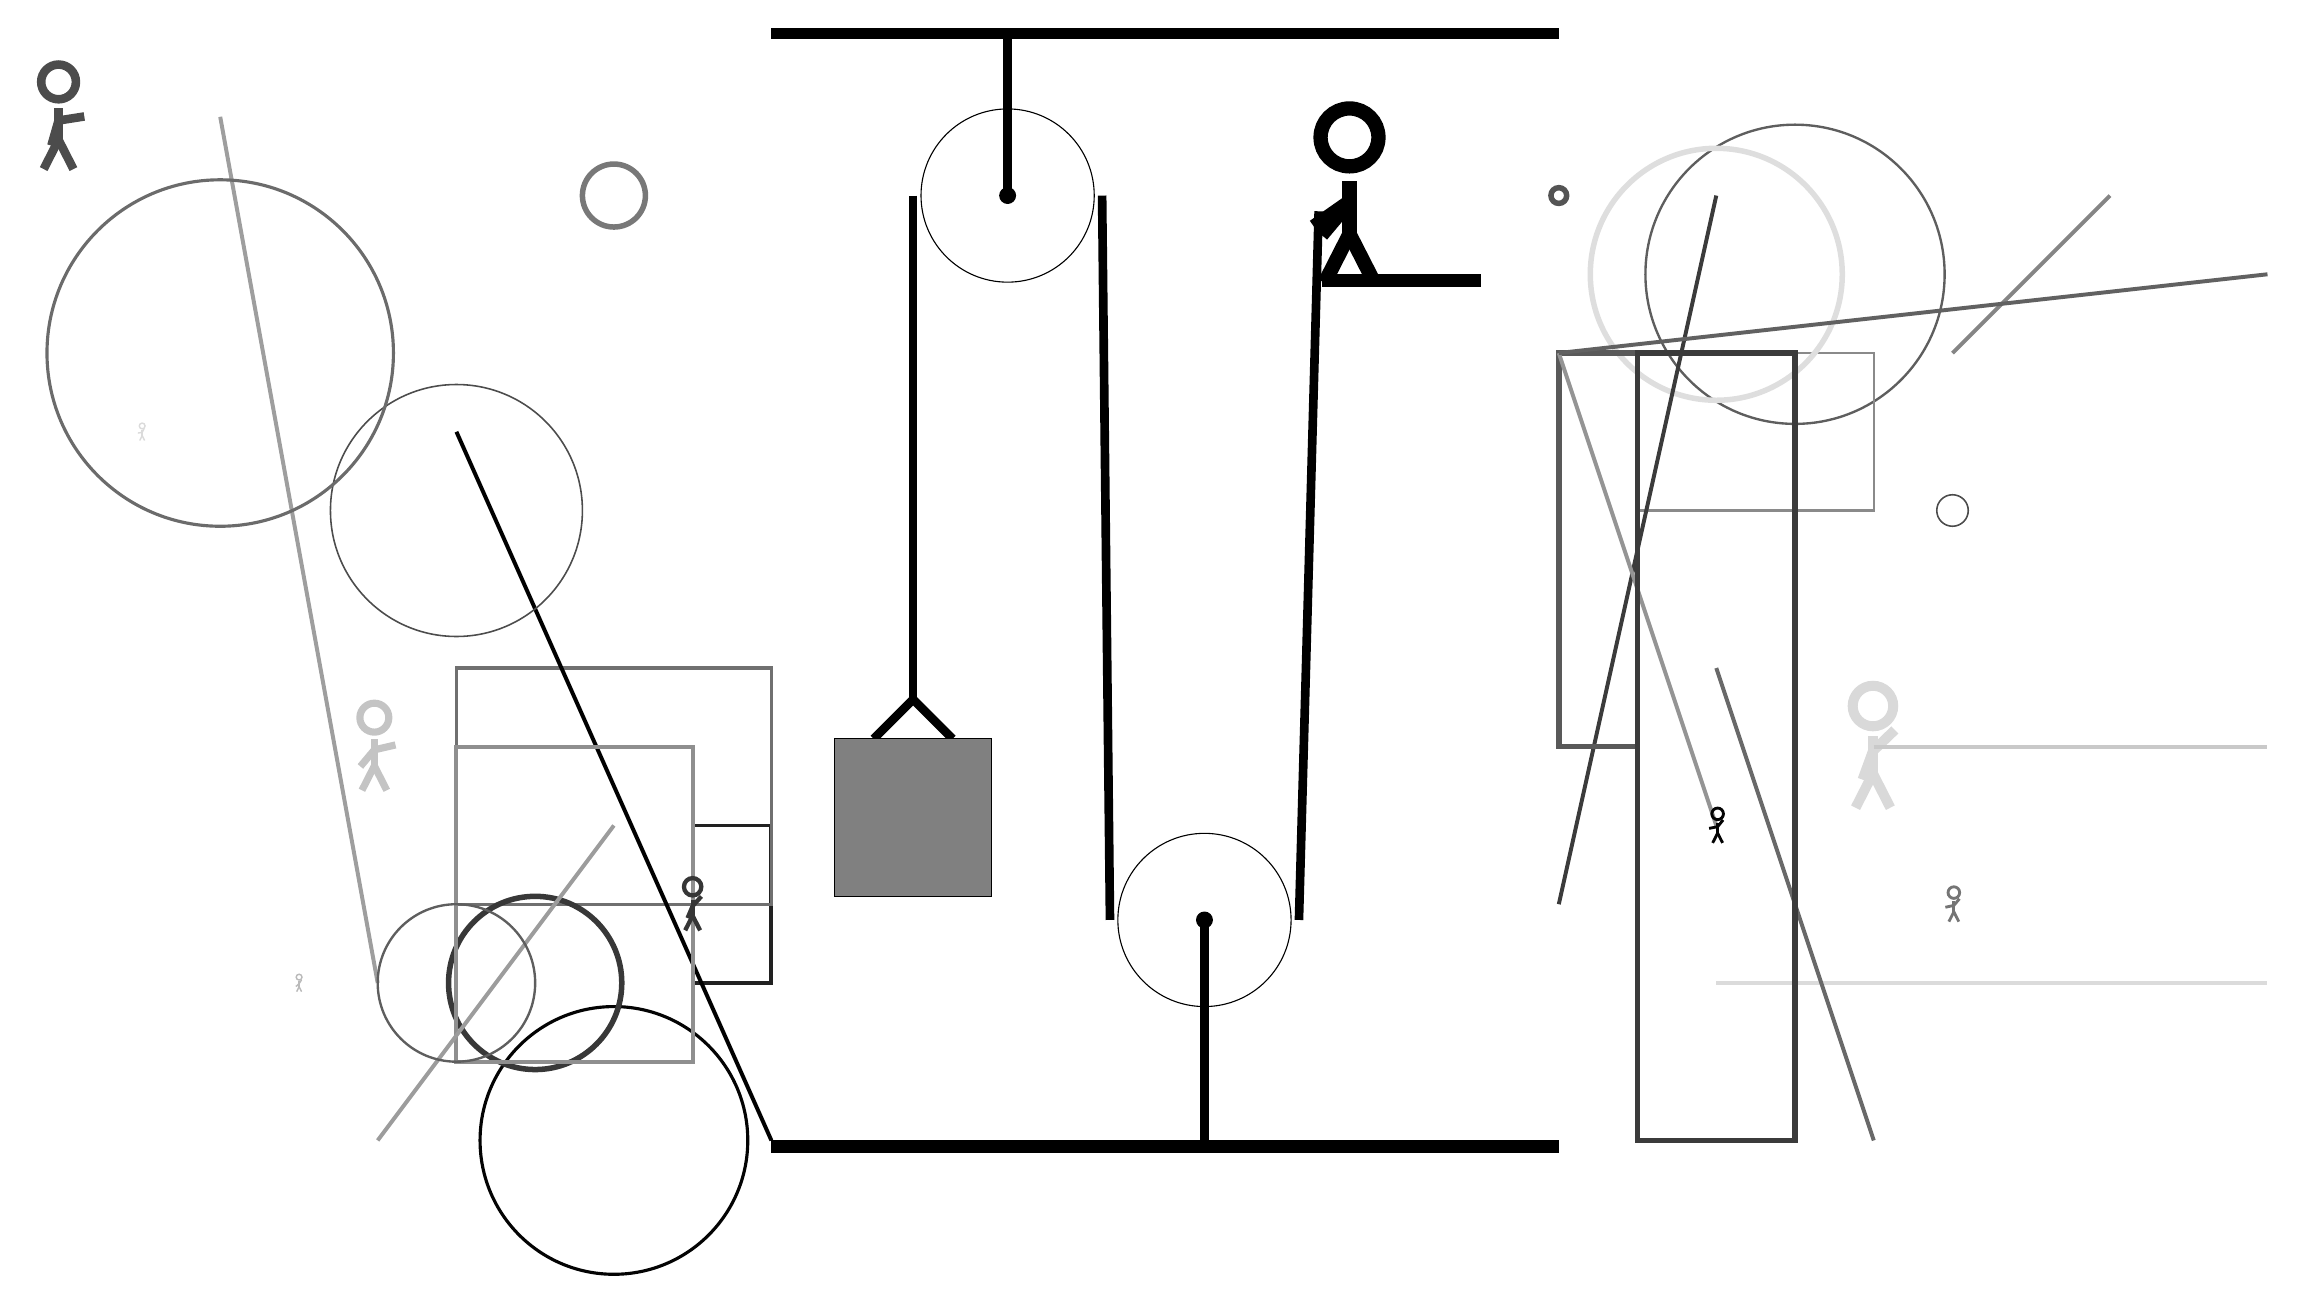
\begin{tikzpicture}
			%%%%% START %%%%%
			
			\draw[fill=black] (-2, 14) rectangle (8, 14.125);
			
			\draw (3.5, 2.8) circle (1.1);
			\draw[fill=black] (3.5, 2.8) circle (0.1);
			\draw[line width=1.1mm] (3.5, 2.8) -- (3.5, 0);
			
			\draw (1, 12) circle (1.1);
			\draw[fill=black] (1, 12) circle (0.1);
			\draw[line width=1.1mm] (1, 14) -- (1, 12);
			
			\draw[line width=1.1mm](-0.7, 5.1) --  (-0.2, 5.6) -- (0.3, 5.1);
			\draw[fill=black!50] (-1.2, 5.1) rectangle (0.8, 3.1);
			
			\draw[line width=1.1mm](-0.2, 12) -- (-0.2, 5.6);
			\centerarc[line width=1.1mm](1, 12)(180:0:1.2000000000000002)
			\draw[line width=1.1mm](2.2, 12) -- (2.3, 2.8);
			\centerarc[line width=1.1mm](3.5, 2.8)(180:360:1.2000000000000002)
			\draw[line width=1.1mm](4.7, 2.8) -- (4.95, 11.8);
			
			\draw[line width=0.5mm, color=black!87] (-3, 4) rectangle (-2, 2);
			
			\draw [line width=0.3mm, color=black!63](11, 11) circle (1.9);
			\draw [line width=0.7mm, color=black!67](8, 12) circle (0.1);
			\node[line width=0.2mm, color=black!23] at (-7, 5) {\Strichmaxerl[5][50][13]};
			\draw [line width=0.4mm, color=black!99](-4, 0) circle (1.7);
			
			\draw[line width=0.4mm, color=black!56] (-2, 6) rectangle (-6, 3);
			\node[line width=0.3mm, color=black!15] at (12, 5) {\Strichmaxerl[7][70][44]};
			\draw [line width=0.7mm, color=black!78](-5, 2) circle (1.1);
			\draw[line width=0.3mm, color=black!46] (9, 10) rectangle (12, 8);
			\draw [line width=0.7mm, color=black!13](10, 11) circle (1.6);
			\draw[line width=0.5mm, color=black!77](8, 3) -- (10, 12);
			\draw[line width=0.5mm, color=black!14](10, 2) -- (17, 2);
			\draw[line width=0.7mm, color=black!65] (9, 5) rectangle (8, 10);
			
			\draw[line width=0.5mm, color=black!38](-7, 2) -- (-9, 13);
			\draw[line width=0.5mm, color=black!48](13, 10) -- (15, 12);
			\draw[line width=0.5mm, color=black!42](8, 10) -- (10, 4);
			\node[line width=0.2mm, color=black!14] at (-10, 9) {\Strichmaxerl[1][9][63]};
			
			\draw[line width=0.5mm, color=black!100](-6, 9) -- (-2, 0);
			\node[line width=0.4mm, color=black!70] at (-11, 13) {\Strichmaxerl[6][74][9]};
			\node[line width=0.5mm, color=black!99] at (10, 4) {\Strichmaxerl[2][11][51]};
			\draw[line width=0.5mm, color=black!62](8, 10) -- (17, 11);
			\draw [line width=0.7mm, color=black!53](-4, 12) circle (0.4);
			\draw[line width=0.5mm, color=black!44] (-3, 5) rectangle (-6, 1);
			\draw [line width=0.2mm, color=black!70](-6, 8) circle (1.6);
			\draw[line width=0.5mm, color=black!30](10, 7) -- (10, 7);
			\draw[line width=0.5mm, color=black!39](-7, 0) -- (-4, 4);
			\node[line width=0.2mm, color=black!79] at (-3, 3) {\Strichmaxerl[3][67][48]};
			\node[line width=0.2mm, color=black!54] at (13, 3) {\Strichmaxerl[2][12][50]};
			\draw [line width=0.3mm, color=black!63](-6, 2) circle (1.0);
			\node[line width=0.7mm, color=black!27] at (-8, 2) {\Strichmaxerl[1][43][56]};
			\draw [line width=0.4mm, color=black!58](-9, 10) circle (2.2);
			
			\draw[line width=0.5mm, color=black!59](10, 6) -- (12, 0);
			\draw[line width=0.5mm, color=black!21](12, 5) -- (17, 5);
			\draw [line width=0.2mm, color=black!70](13, 8) circle (0.2);
			\draw[line width=0.7mm, color=black!77] (9, 0) rectangle (11, 10);
			
			\node at (5.3, 12) {\Strichmaxerl[10][35][-130]};
			\draw[fill=black] (5, 11) rectangle (7, 10.85);
			
			\draw[fill=black] (-2, 0) rectangle (8, -0.15);
			
			%%%%% END %%%%%
		\end{tikzpicture}
	\end{figure}	
\end{document}